\section{Operationsverstärker \formelbuch{3}}
	\subsection{Opamp Schaltungen}
		\subsubsection{Invertierender Verstärker \formelbuch{3-7}}
			Beim invertierenden Verstärker ist die Ausgangsspannung gegenphasig
      zur Eingangsspannung.\\
			\begin{minipage}[T]{12cm}
       	\begin{tabular}{ll}
       	Closed-Loop Spannung: & 
       	$A_{CL}=\frac{v_{out}}{v_{in}}=-\frac{R_F}{R_1}$\\
       	& $v_{out} = -v_{in}\cdot\frac{R_F}{R_1}$\\
       	$i_1=\frac{v_{in}+v_d}{R_1}$ & 
      	$i_F=-\frac{v_{out}+v_d}{R_F}$\\
       	Ausgangswiderstand des I-Verstärkers: &
       	$r_{out}=0\Omega$\\
       	Eingangswiderstand des I-Verstärkers: & 
       	$r_{in}=R_1$\\
       	\end{tabular}
      \end{minipage}
			\begin{minipage}{6cm}
       	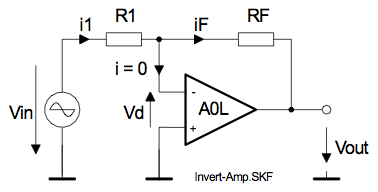
\includegraphics[width=6cm]{./bilder/i-verstaerker.png}
      \end{minipage}\\
      
		\subsubsection{Nichtinvertierender Verstärker \formelbuch{3-10}}
			Beim nichtinvertierenden Verstärker ist die Ausgangsspannung
      gleichphasig zur Eingangsspannung.\\ 
			\begin{minipage}[T]{12cm}
      	
        \begin{tabular}{ll}
        	Closed-Loop Gain: &
        	$A_{CL}=\frac{v_{out}}{v_{in}}=\frac{R_F}{R_1}+1$\\
        	& $v_{out} = v_{in}\cdot(\frac{R_F}{R_1}+1)$ \\
        	$i_1=\frac{v_{in}-v_d}{R_1}$ &
        	$i_F=\frac{v_{out}}{R_F+R_1}$\\
          Ausgangswiderstand des NI-Verstärkers: &
          $r_{out}=0\Omega$\\
          Eingangswiderstand des NI-Verstärkers: &
          $r_{in}=\infty$\\
        \end{tabular}
      \end{minipage}
			\begin{minipage}{6cm}
      	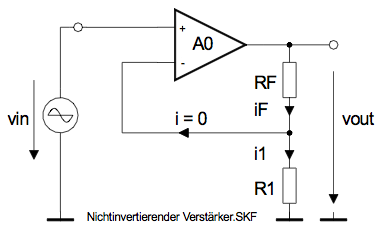
\includegraphics[width=6cm]{./bilder/ni-verstaerker.png}
      \end{minipage}\\

		\subsubsection{Verstärker mit mehreren Eingängen \formelbuch{3-12}}
			\begin{minipage}{12.5cm}
            	$A_{CL1}=-\frac{R_F}{R_1}$\\
            	$A_{CL2}=-\frac{R_F}{R_2}$\\
            	$A_{CL3}=\frac{R_F+(R_1//R_2)}{(R_1//R_2)}$\\
            	$v_{out}=A_{CL1}v_1+A_{CL2}v_2+A_{CL3}v_3=
            	-\frac{R_F}{R_1}v_1-\frac{R_F}{R_2}v_2+\frac{R_F+(R_1//R_2)}{(R_1//R_2)}$\\
      \end{minipage}
			\begin{minipage}{5.5cm}
      	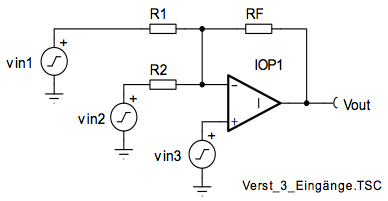
\includegraphics[width=5.5cm]{./bilder/3-eingaenge.png}
      \end{minipage}\\

		\subsubsection{Invertierender Addierer \formelbuch{3-20}}
			\begin{minipage}[b]{12cm}
            $V_{out}=A_{CL1}V_{IN1}+A_{CL2}V_{IN2}+\ldots$\\
            $V_{out}=- \frac{R_F}{R_1}V_{IN1}- \frac{R_F}{R_2}V_{IN2}+\ldots$\\
            $A_{CL1}=- \frac{R_F}{R_1}$\\
           	$A_{CL2}=- \frac{R_F}{R_2}$\\
      \end{minipage}
			\begin{minipage}{6cm}
      	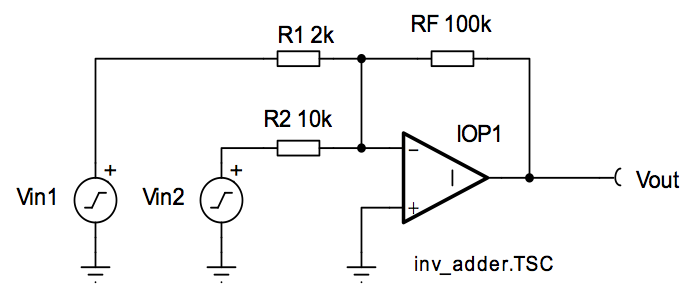
\includegraphics[width=6cm]{./bilder/invertadd.png}
      \end{minipage}\\

		\subsubsection{Gewichteter Subtrahierer \formelbuch{3-20}}
			\begin{minipage}[b]{12cm}
            	$A_{CL1}=- \frac{R_F}{R_1}$\\
            	$A_{CL2}=
           		\frac{R_3}{R_3+R_2}\left(1+\frac{R_F}{R_1}\right)$\\
            	$v_{out}=
            	\frac{R_3}{R_3+R_2}\left(1+\frac{R_F}{R_1}\right)
            	v_{in2}-\frac{R_F}{R_1}v_{in1}$\\
      	\end{minipage}
			\begin{minipage}{6cm}
            	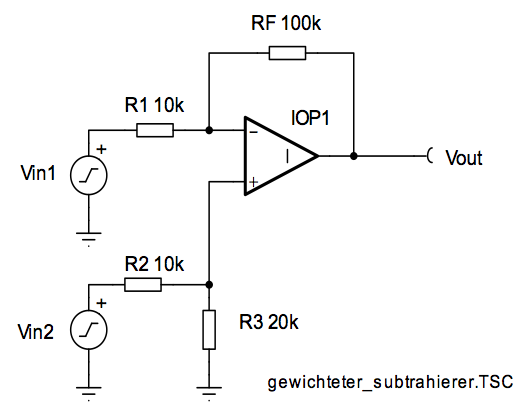
\includegraphics[width=6cm]{./bilder/gewichtsub.png}
            \end{minipage}\\


		\subsubsection{Mehrfach-Addierer-Subtrahierer \formelbuch{3-23}} 		
		\begin{minipage}[b]{12cm}
		1. Man waehlt $R_{F}$\\
		2. Man waehlt $R_{P}$, wobei oft $R_{P}=R_{F}$ gesetzt wird. (optional)\\
		3. $R_{n}=\frac{R_{F}}{\left|A_{n}\right|}$ oder
			$R_{n}=\frac{R_{P}}{\left|A_{n}\right|}$\\ 
		4. Verstärkungsbedingung: $A_{N1} +
		\ldots + A_{Nn} = A_{P1} + \ldots + A_{Pn}$ \\Falls unerfüllt, muss ein Dummyeingang hinzugefügt werden!
		\end{minipage}
		\begin{minipage}{6cm}
          	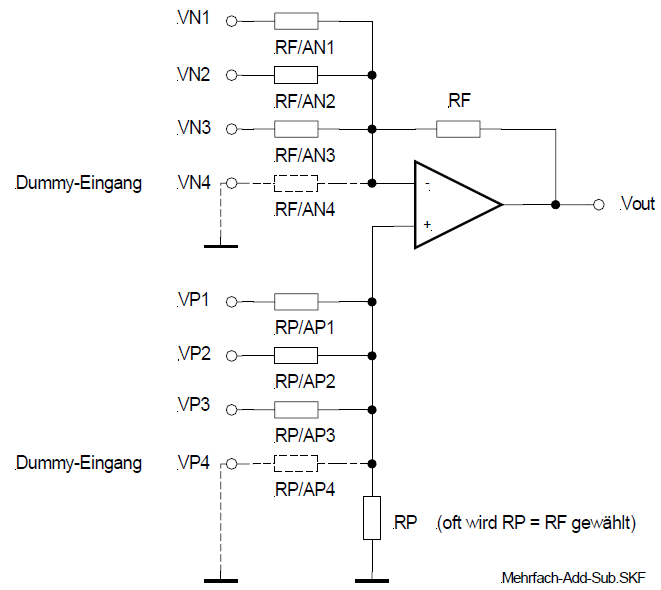
\includegraphics[width=6cm]{./bilder/mehrfach-addierer-subtrahierer.png} 
        \end{minipage}\\

		\subsubsection{Instrumentenverstärker \formelbuch{3-25}}
		\begin{minipage}[b]{12cm}
		$A_{diff}=\frac{V_{out}}{V_{diff}}=\frac{V_{P}-V_{N}}{V_{inP}-V_{inN}}
		=\frac{2R_{1}+P}{P}=\frac{2R_{1}}{P}+1$\\
		\end{minipage}
		\begin{minipage}{6cm}
          	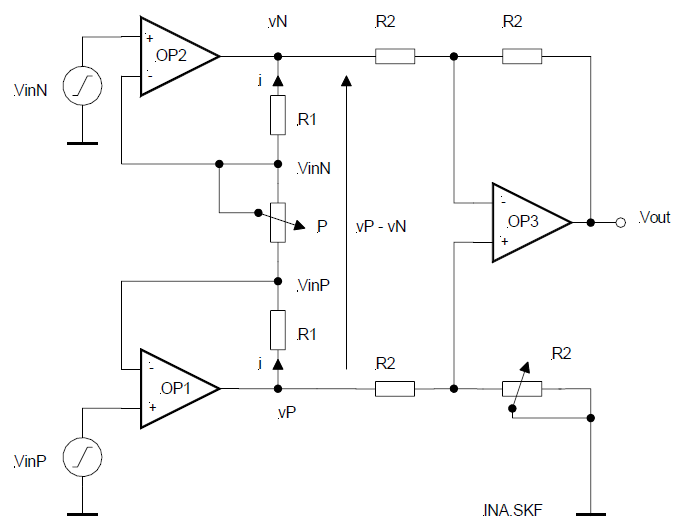
\includegraphics[width=6cm]{./bilder/Instrumentationsverstaerker.png} 
        \end{minipage}\\

		\subsubsection{Differenzverstärker \formelbuch{3-21}}
			\begin{minipage}[b]{12cm}
            	$A_{diff}=\frac{v_{out}}{(v_{in2}-v_{in1})}$\\
            	$v_{out} = \frac{R_F}{R_1}\cdot (v_{in2}-v_{in1})$\\
            	Widerstandsbedingung für den Differenzverstärker\\
            	$A_{diff}=\frac{R_F}{R_1}=\frac{R_3}{R_2}$\\
            \end{minipage}
			\begin{minipage}{6cm}
            	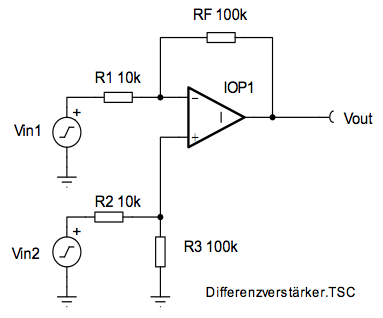
\includegraphics[width=6cm]{./bilder/differenzver.png}
            \end{minipage}\\


		\subsubsection{Komparatorschaltung \formelbuch{3-27}}
			\begin{minipage}{18cm}
            	Wenn ein Operationsverstärker als {\it Verstärker ohne
            	Gegenkopplung} betrieben wird, spricht man von einer {\it
            	Komparatorschaltung}. Der Operationsverstärker wird dann als {\it
            	Komparator} betrieben.\\
            	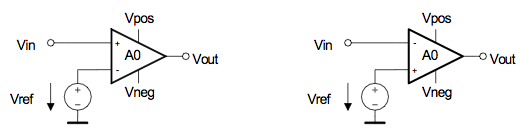
\includegraphics[width=16cm]{./bilder/komparator.png}\\
            	Beim nichtinvertierenden Komparator (links)\\
            	$V_{out}=V_{out\hspace{1mm}max}=V_{pos}-V_{Rand}
            	\mbox{ wenn } V_{in} > V_{ref}\pm V_{OS} \mbox{ bzw. } 
            	V_{diff}\pm V_{OS}>0$\\
            	$V_{out}=V_{out\hspace{1mm}min}=V_{neg}+V_{Rand}
            	\mbox{ wenn } V_{in} < V_{ref}\pm V_{OS} \mbox{ bzw. } 
            	V_{diff}\pm V_{OS}<0$\\ \\
            	Beim invertierenden Komparator (rechts)\\
            	$V_{out}=V_{out\hspace{1mm}max}=V_{pos}-V_{Rand}
            	\mbox{ wenn } V_{in} < V_{ref}\pm V_{OS} \mbox{ bzw. } 
            	V_{diff}\pm V_{OS}<0$\\
            	$V_{out}=V_{out\hspace{1mm}min}=V_{neg}+V_{Rand}
            	\mbox{ wenn } V_{in} > V_{ref}\pm V_{OS} \mbox{ bzw. } 
            	V_{diff}\pm V_{OS}>0$\\
            \end{minipage}

		\subsubsection{Schmitt-Trigger \formelbuch{3-31}}
		Nichtinvertierender Schmitt-Trigger\\
			\begin{minipage}{9cm}
	          	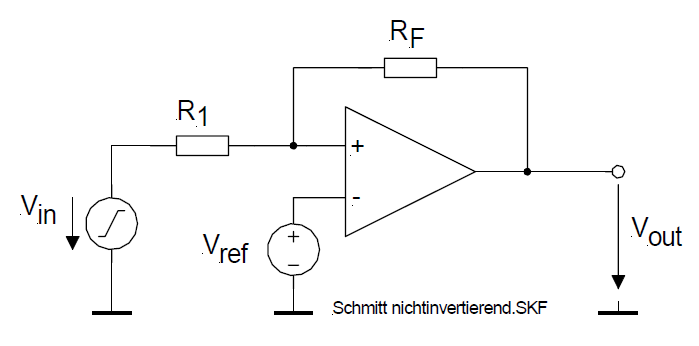
\includegraphics[width=8cm]{./bilder/n-schmitt.png} 
	        \end{minipage}
			\begin{minipage}{9cm}
	          	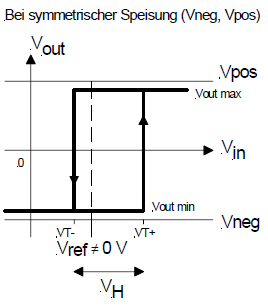
\includegraphics[width=4cm]{./bilder/n-schmitt-kennlinie.png} 
	        \end{minipage}\\
		Invertierender Schmitt-Trigger\\
			\begin{minipage}{9cm}
	          	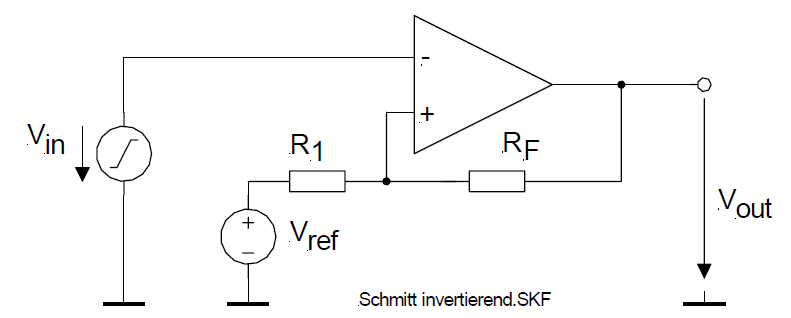
\includegraphics[width=8cm]{./bilder/i-schmitt.png} 
	        \end{minipage}
			\begin{minipage}{9cm}
	          	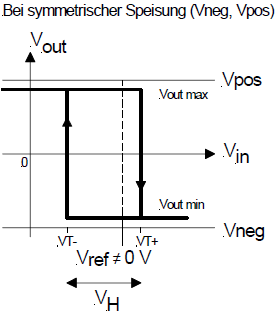
\includegraphics[width=4cm]{./bilder/i-schmitt-kennlinie.png} 
	        \end{minipage}\\
			
			\begin{minipage}{18cm}
               	Hysteresespannung:\\
               	\hspace*{10mm}
               	\begin{tabular}{| c | c |}
                \hline
                Nichtinvertierender Schmitt-Trigger & Invertierender
                Schmitt-Trigger\\
                \hline
                $V_H=(V_{out \hspace{1mm} max}-V_{out \hspace{1mm}
                min})\frac{R_1}{R_F}$ &
                $V_H=(V_{out \hspace{1mm} max}-V_{out \hspace{1mm}
                min})\frac{R_1}{R_1+R_F}$\\
                \hline
            \end{tabular}\\ \\
				Schwellspannung:\\
				\hspace*{10mm}
			\begin{tabular}{| c | c |}
                \hline
                Nichtinvertierender Schmitt-Trigger & Invertierender
                Schmitt-Trigger\\
                \hline
                $V_{T+}=V_{ref}+(V_{ref}-V_{out
                \hspace{1mm} min})\frac{R_1}{R_F}$ &
                $V_{T+}=V_{ref}+(V_{out \hspace{1mm}
                max}-V_{ref})\frac{R_1}{R_1+R_F}$\\
                \hline
                $V_{T-}=V_{ref}-(V_{out
                \hspace{1mm} max}-V_{ref})\frac{R_1}{R_F}$ &
                $V_{T-}=V_{ref}-(V_{ref}-V_{out \hspace{1mm}
                min})\frac{R_1}{R_1+R_F}$\\
                \hline
            \end{tabular}\\
            \end{minipage}
	
		\subsubsection{Differentiator \formelbuch{3-42}}
			\begin{minipage}[b]{12cm}
           		Beim Differentiator gilt $v_{out}=v_N-i_1 \cdot R_F$ wobei
           		$v_N=0$\\
           		$i_1=C_1 \cdot \frac{dv_C}{dt}$\\
           		$v_{out}=-R_FC_1 \frac{dv_{in}}{dt}$\\
           		Die Elemente $C_F$ und $R_1$ sind optional. \\
           		Sie beheben jedoch Probleme die ohne \\
           		sie entstehen (siehe elemenarer Differentieator). \\
           		Mit $C_F$ und $R_1$: \\
           		- Keine differentiation bei hoeheren Frequenzen. \\
           		- Limitierte Verstaerkuing bei hoeheren Frequenzen. \\
           		- Eingangswiderstand immer groesser $R_1$ \\ 
           		$\rightarrow$ keine Belastung der Signalquelle
           
           	\end{minipage}
			\begin{minipage}{6cm}
           		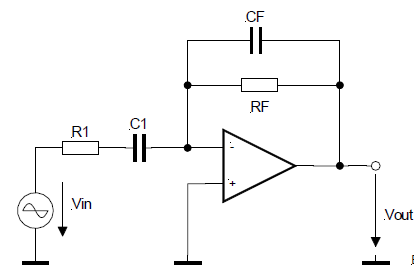
\includegraphics[width=6cm]{./bilder/differentiator.png}
           	\end{minipage}

		\subsubsection{Integrator \formelbuch{3-45}} 
		\vspace{1cm}
		\begin{minipage}[b]{12cm}
		$v_{out}=-\frac{1}{RC} \int{v_{in}}dt +
		v_{out\hspace{1mm}Anfang} $\\
		$\frac{dv_{out}}{dt}=-\frac{v_{in}}{RC}$\\
		\end{minipage} 
		\begin{minipage}{6cm}
          	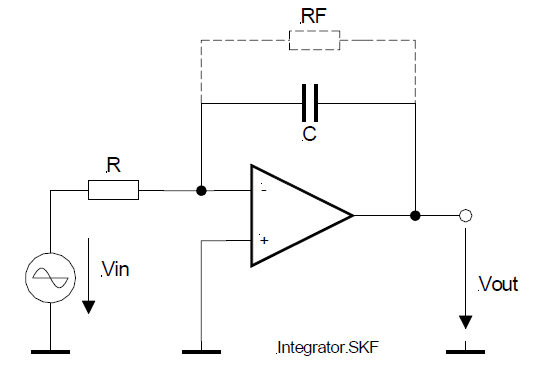
\includegraphics[width=6cm]{./bilder/integrator.png} 
        \end{minipage}\\

		\subsection{Fehlereinflüsse des Opamp \formelbuch{3-51}}
		\subsubsection{Verstärkungsfehler bei endlicher Closed-Loop-Verstärkung
		\formelbuch{3-51}}
			\begin{minipage}{12cm}
				\begin{tabular}{ll}
               	beim nichtinvertierenden Verstärker &
               	$A_{CL \hspace{1mm} ideal}=\frac{R_F}{R_1}+1$\\
               	beim invertierenden Verstärker &
                $A_{CL \hspace{1mm}
               	ideal}=-\frac{R_F}{R_1}$\\
         \end{tabular}
               	Beim invertierenden Verstärker ist eine kleine Korrektur
               	anzubringen: \\
               	$\frac{1}{A_{CL \hspace{1mm}
               	real}}=\frac{1}{A_{CL \hspace{1mm} real}}+\frac{1}{nA_{OL}}$\\
	        \end{minipage}
			\begin{minipage}{6cm}
               	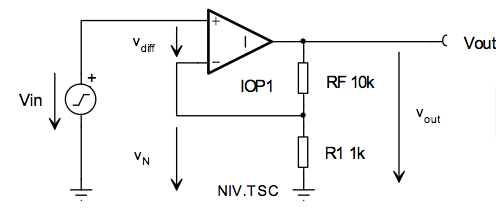
\includegraphics[width=6cm]{./bilder/verstaerkungsfaktor.png}
            \end{minipage}

		\subsubsection{Common-Mode-Fehler \formelbuch{3-60}}
				\begin{tabular}{llll}
					Mittelspannung: &
					$V_M=\frac{V_{pos}+V_{neg}}{2}$ &
					Opamp-Eingangsspannung: &
					$V_{OP\ IN}=\frac{V_P+V_N}{2}$\\					
					Offsetspannung: &
					$V_{OS}=\frac{V_{CM}}{CMRR_{lin}}$ &
					Ausgangs-Fehlerspannung: &
					$V_{out \hspace{1mm} E}=\left|V_{OS}\right| \cdot A_{CL+}=\left|
					\frac{\Delta V_{CM}}{CMRR_{lin}}\right|A_{CL+}$\\
				\end{tabular}
				
				\begin{tabular}{ll}
        	Common-Mode-Spannung: &
          $V_{CM}=V_{OP \hspace{1mm} IN}-V_M=V_P- \frac{V_{pos}+V_{neg}}{2} \mbox{ bzw. }V_N- \frac{V_{pos}+V_{neg}}{2}$\\
          & $V_{CM}\frac{V_{P}+V_{N}}{2}-V_M$ \\
          Lineare Definition: &
          $CMRR_{lin}=\frac{dV_{CM}}{dV_{OS}}=10^{\frac{CMRR_{dB}}{20}}=\frac{A_{OL}}{A_{CM}}$\\
          Logarithmische Definition: &
          $CMRR_{dB}=20 \cdot log(CMRR_{lin})=20 \cdot
          log\frac{dV_{CM}}{dV_{OS}}$\\
				\end{tabular}
		
		\subsubsection{Offsetspannungsfehler \formelbuch{3-53}}
				\begin{tabular}{ll}
					Im Closed-Loop-Betrieb ist die Ausgangs-Fehlerspannung: &
					$V_{out \hspace{1mm}E}=V_{OS}\left( 1+\frac{R_F}{R_1}\right)$\\
          allgemein: &
          $V_{out \hspace{1mm}E}=V_{OS} \cdot {A_{CL}}^{+}$\\
          Im Open-Loop-Betrieb ist die Ausgangs-Fehlerspannung: &
          $V_{out \hspace{1mm}E}=V_{OS}\cdot {A_{CL}}^{+}$\\
         \end{tabular}
		
		\subsubsection{Eingangsstromfehler \formelbuch{3-54}}
			\begin{minipage}{18cm}
              Wenn die Opamp-Eingangsströme gleich gross sind
              ($I_{N}=I_{P}$) und die Gleichstromwiderstände,
              die von jedem Opamp-Eingang nach Masse führen, 
              ebenfalls gleich gross gewählt werden, heben sich die
              Ausgangsspannungsfehler, die durch $I_{N}$ und $I_{P}$
              erzeugt werden, gegenseitig auf. \\
              \begin{tabular}{ll}
              Allgemeine Formel für den
              Eingangsstromfehler: &
              $V_{out \hspace{1mm}E}=I_N R_F-R_2 I_P\left( 1+\frac{R_F}{R_1} \right)$\\
              Widerstandsbedingung für Eingangsstromkompensation:&
              $R_2=\frac{R_F R_1}{R_F+R_1}=R_F // R_1$\\
            	\end{tabular}
            \end{minipage}\\
			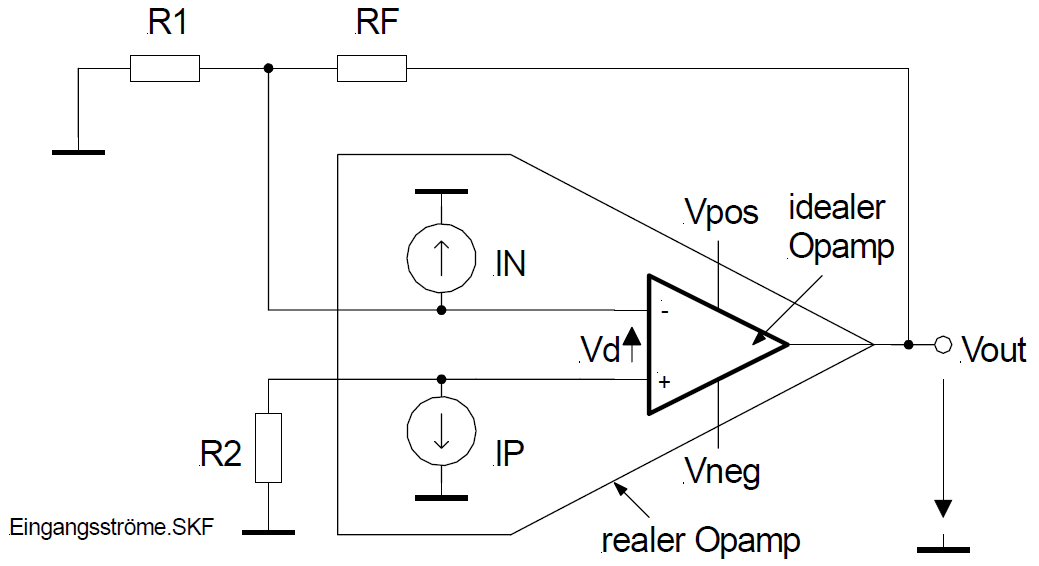
\includegraphics[width=8cm]{./bilder/eingangsstromfehler.png}

		\subsubsection{Eingangsstromkompensation ohne AC-Zweige \formelbuch{3-54}}
			\begin{minipage}[b]{6cm}
            	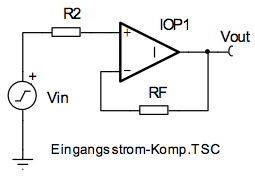
\includegraphics[height=3cm]{./bilder/spannungsfolger.png}\\
            	\centerline{{\bf Spannungsfolger}}\\ \\
            	$R_2$ sei ein gegebener Quellen-Widerstand\\
            	{\bf $R_F$ muss eingefügt werden}\\ \\
            	$R_F=R_2$
            \end{minipage}\hfill
			\begin{minipage}[b]{6cm}
            	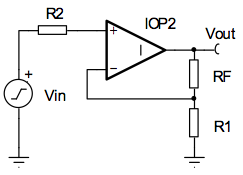
\includegraphics[height=3cm]{./bilder/nichtinver}\\
            	\centerline{{\bf Nichtinvertierender Verstärker}}\\ \\
            	Hier sei der Quellenwiderstand
            	vernachlässigbar.\\ {\bf $R_2$ muss eingefügt werden}\\ \\
            	$R_2=R_F//R_1$
            \end{minipage}\hfill
			\begin{minipage}[b]{6cm}
            	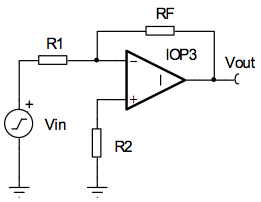
\includegraphics[height=3cm]{./bilder/inver}\\
            	\centerline{{\bf Invertierender Verstärker}}\\ \\ \\ \\
            	{\bf $R_2$ muss eingefügt werden}\\ \\
            	$R_2=R_F//R_1$
            \end{minipage}
			\begin{minipage}{18cm}
            	\vspace{3mm}
				\textbf{Ausgangsspannungsfehler} auf Grund des \textbf{Offsetstromes} (nur bei
				Kompensation(!)):
				\fbox{$V_{out \hspace{1mm}E}=\left|I_{OS}\right| \cdot R_F$}\\
			\end{minipage}

		\subsubsection{Power-Supply-Fehler \formelbuch{3-58}}
            Die grösse $PSRR$ (Power Supply Rejection Ratio, Speisespannungsunterdrückung)\\
            \begin{tabular}{ll}
            Offsetspannung:&
            $V_{OS}=\frac{\Delta V_{Supply}}{PSRR_{lin}}$\\
            Ausgangsspannungsfehler:&
            $V_{out \hspace{1mm}E}=\left|V_{OS}\right| A_{CL+}=\left| \frac{\Delta V_{Supply}}{PSRR_{lin}}\right| A_{CL+}$\\
            Lineare Definition: &
            $PSRR_{lin}=\frac{dV_{Supply}}{dV_{OS}}=10^{\frac{PSRR_{dB}}{20}}$\\
            Logarithmische Definition:&
            $PSRR_{dB}=20 log PSRR_{lin}=20 log \frac{dV_{Supply}}{dV_{OS}}$\\
            \end{tabular}
            

		\subsubsection{Zusammenfassung aller Fehlereinflüsse \formelbuch{3-63}}
      $V_{out\hspace{1mm}E\hspace{1mm}total}=A_{CL+}\cdot\left[\left|V_{OS}\right|+\frac{\left|V_{CM}\right|}{CMRR}
            	+\frac{\left|\Delta V_{Supply}\right|}{PSRR}\right]+\left|I_{OS}\right|R_F$\\

		\subsection{Dynamische Eigenschaften des Opamp \formelbuch{3-66}}
			\begin{tabular}{ll}
				dB-Verstärkung:&
        $A_{dB}=20 \cdot log A_{lin}$\\
        lineare Verstärkung:&
        $A_{lin}=10^{\frac{A_{dB}}{20}}$\\
			\end{tabular}
      Verstärkungs-Bandbreite-Produkt GBP (Gain-Bandwidth-Product)\\
      \begin{tabular}{ll}
        Bandbreite des gegengekoppelten {\it nichtinvertierenden} Verstärkers:&
        $f_{CL+}=\frac{GBP}{A_{CL \hspace{1mm}lin}}$\\
        Bandbreite des gegengekoppelten {\it invertierenden} Verstärkers: &
        $f_{CL}=\frac{GBP}{\left| A_{CL \hspace{1mm}lin}\right|+1}$\\
      \end{tabular}
      {\bf Gesetz vom Konstanten Verstärkungs-Bandbreite-Produkt:} \\ \\
      	Für jeden Punkt auf der mit -20dB abfallenden Frequenzgang-Gerade ist das
        Produkt aus Verstärkung und zugehöriger Frequenz konstant gleich GBP, d.h. $A_{lin}\cdot f=GBP=konst$\\
      
		\subsubsection{Slew-Rate}
		\begin{tabular}{ll}
			min. SR bei einem Sprungsignal &
			$SR\geq\frac{0.8V_{step}}{t_{anstieg}}$\\ 
			min. SR bei einem Sinussignal & 
			$SR\geq V_{amplitude}\omega=V_{amplitude}2\pi f$\\
		\end{tabular}

		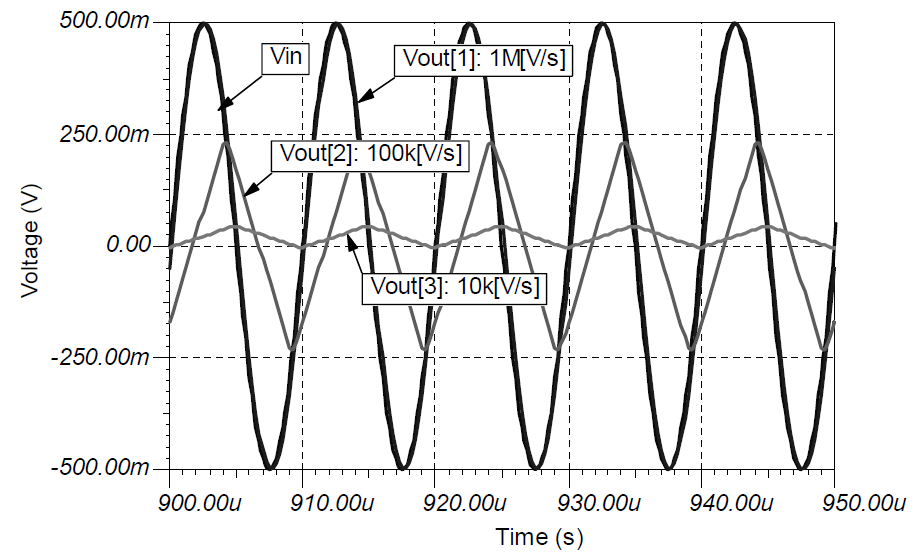
\includegraphics[height=5cm]{./bilder/slew-rate.png}\\